\section{Conclusions}
The suite of simulations showed that constellations with higher altitude or a higher number of satellites provided more raw coverage time. A higher altitude allowed for a greater sensor footprint, meaning that a trans-oceanic flight would stay `in-view' for longer. Having more satellites simply increases the probability of a satellite being above a trans-oceanic flight at any one point in time.

Despite the geographic coverage performance of high altitude constellations, low altitude constellations showed a marked improvement in signal performance. Lower altitudes represented less distance required to travel by any one ADS-B transmission, resulting in lower signal loss. This effect was dramatic enough such that the lowest altitude constellation performed better than most other constellations as seen in Table \ref{tab:decMatRes}.

The inclination trend analysis suggested that a constellation with all satellites inclined at 90 degrees may represent the best coverage trade-off between the three flights. This inclination represents the best possible geometric configuration for full global coverage. However, the nature of one-dimensional parameter variance in the tests conducted and the weighted decision matrix meant that the 90 degree inclination configuration did not feature in the `best choices'. 
\subsection{Chosen Constellation}
The results from the weighted decision matrix show that a satellite constellation with parameters as defined in Table \ref{tab:18sat_winner} is the best performing space based ADS-B system of those tested. This particular constellation performed strongly in being able to provide a high level of coverage for the three trans-oceanic flights studied in this thesis. A 3D model of this constellation is shown in Figure \ref{fig:18sat_3D} and the ground tracks in Figure \ref{fig:18sat_groundtrack}

% Table generated by Excel2LaTeX from sheet 'Sheet2'
\begin{table}[htbp]
  \centering
  \caption{18 satellite configuration with the best score}
    \begin{tabular}{lr}
    \toprule
    Parameter & Value \\
    \midrule
    Altitude (km above mean radius of Earth) & 700 \\
    Inclination (deg) & 60 \\
    Number of Planes & 3 \\
    Plane Separation (deg RAAN) & 120 \\
    Number of Satellites per plane & 6 \\
    True Anomaly Separation (deg) & 60 \\
    Number of Satellites (Total) & 18 \\
    \bottomrule
    \end{tabular}%
  \label{tab:18sat_winner}%
\end{table}%

\begin{figure}[htbp]
	\centering
	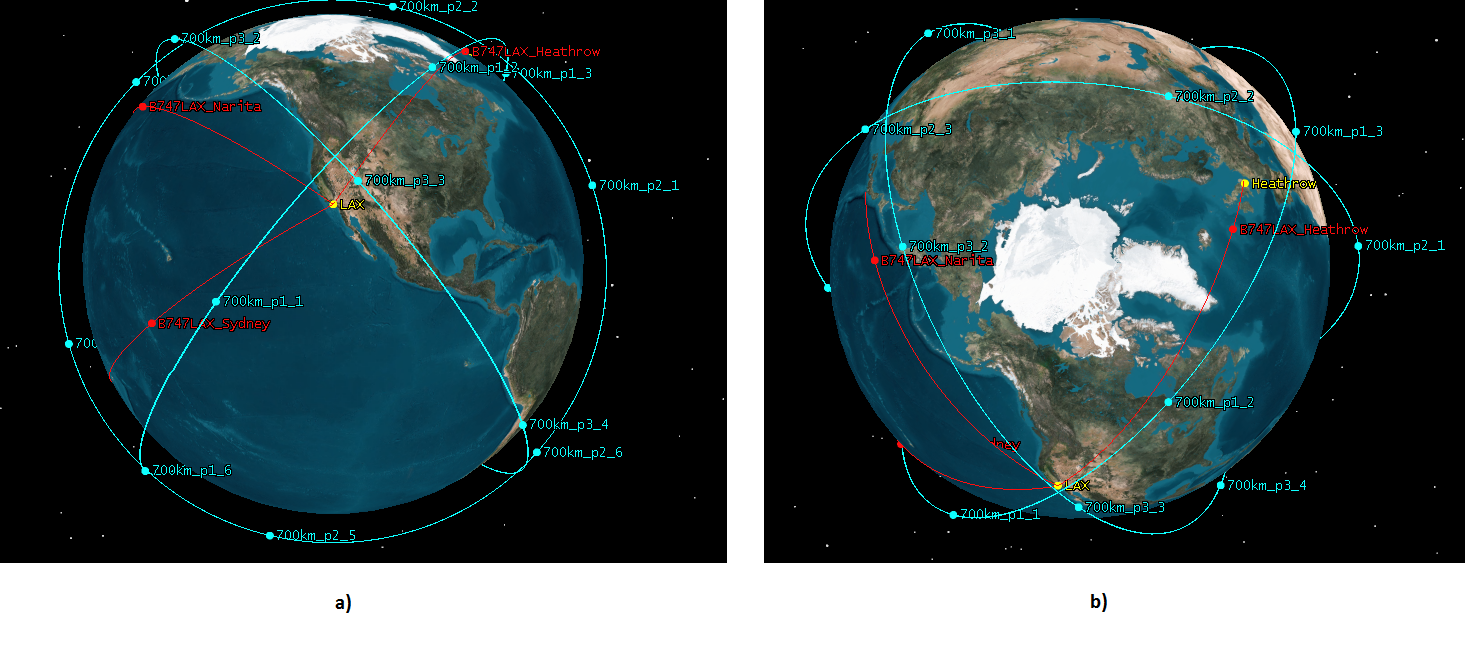
\includegraphics[scale = 0.4]{Pictures/18sat_3D.png}
	
	\caption{18 satellite configuration rendered in STK showing a) the view above North America and b) the view above the Arctic}
	\label{fig:18sat_3D}
\end{figure}

\begin{figure}[htbp]
	\centering
	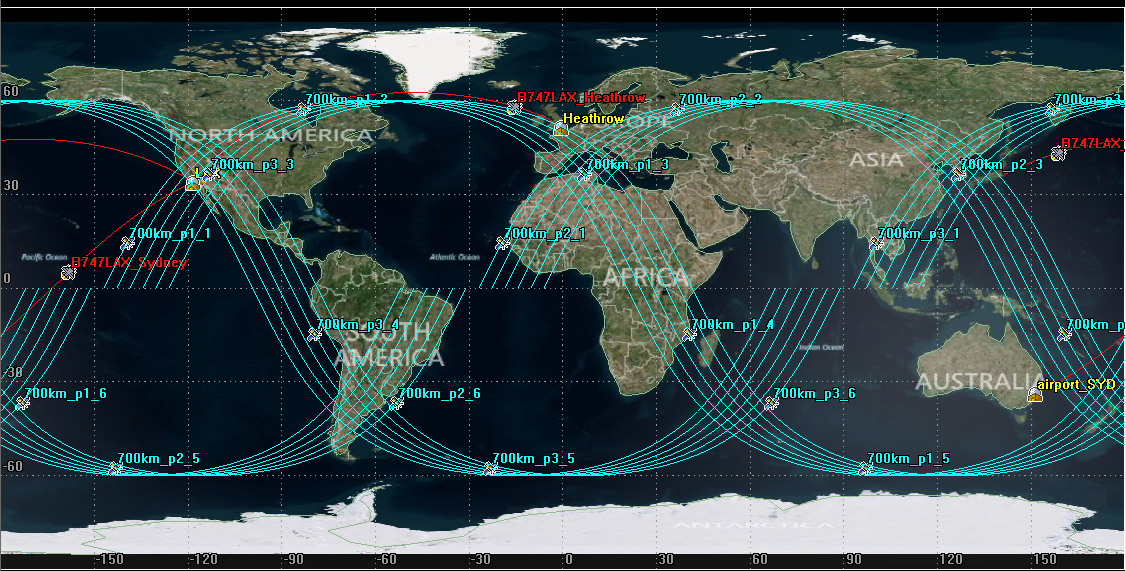
\includegraphics[scale = 0.6]{Pictures/18sat_groundtrack.png}
	
	\caption{Ground track of the 18 satellite configuration, rendered in STK}
	\label{fig:18sat_groundtrack}
\end{figure}

This particular result shows that a higher-number of satellites performs more favourably when considering ADS-B coverage requirements. Interestingly, a lower number of satellites in a lower orbit performs almost as well due to dramatically increased communication link performance. The test conducted only examined variation of one parameter at a time and can not provide a conclusion on whether a combination of two or more parameters would result in the most optimal constellation performance.
